\chapter{Infrastructure}

\section{Hardware}
	\subsection{Sony EVI D100P}
		\begin{figure}[h]
			\centering
			\begin{subfigure}[h]{0.4\linewidth}
				\centering
				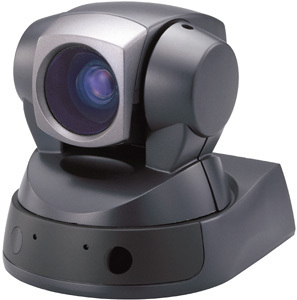
\includegraphics[width=1.6in]{images/ptz_front}
				\caption{Front side.}
			\end{subfigure}
			\qquad
			\begin{subfigure}[h]{0.4\linewidth}
				\centering
				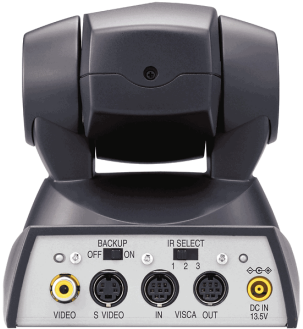
\includegraphics[width=1.6in]{images/ptz_back}
				\caption{Back side.}
			\end{subfigure}
			\caption{Sony EVI D100P.}
			\label{fig:3_evi}
		\end{figure} 
		
		The first hardware element that we used is the Sony EVI D100P\footnote{\url{https://pro.sony/en_IN/products/ptz-network-cameras/evi-d100-d100p-pal-}}. It is a \emph{PTZ} cam (which stands for \emph{Pan Tilt Zoom}). It is a camera which, originally thought and designed for videoconferences, is equipped with a bunch of precision motors. This allows it to be teleoperated, performing a soft and steady two-dimensional movement on demand:
		\begin{itemize}
			\item \emph{Pan:} horizontal movement. It can take values from $-164º$ to $164º$ from the centered position. This movement can be performed at a certain speed, which can be setted between $1$ and $24$.

			\item \emph{Tilt:} vertical movement. Its range goes from $-30º$ to $30º$, and the movement speed can be also varied between $1$ and $20$.
		\end{itemize}

		The low-level implementation of the movement commands is the \emph{VISCA} protocol, a propietary solution from the manufacturer (Sony). It is received by the cam through a RS-232C (the traditional low-rate serial interface before USB extended), so we can connect it to a modern computer with a RS232-USB interface.

		However, the driver that controls this camera (\ref{sec:3_evicam_driver}) does not offer support for a \emph{zoom} movement, but it is not very relevant for this application.\\

		As the video sensor is an analogue device, we need to convert it to a digital format. We achieve this with a video capture device, which outputs video in a digital format. This image flow will be processed by a ROS driver (\autoref{sec:3_usb_cam}), that will be later explained.\\

		Something remarkable about this device is that it is a bidirectional device: we \textit{receive} images from its camera, and, at the same time, we \textit{send} it commands to move the motors.\\
		
		As we can infer from the described technical specifications, this is a relatively old device, so we have to be careful on the movement commands. This is due to the short period of position update: even if we command the motion action at the maximum available speed, the movement won't complete before the next update is commanded. In addition, the camera mantains a buffer of the pending commands to be updated. Hence, sending absolute movement commands (\autoref{fig:3_ptz_wrong}) will result in a chaotic behavior of the camera.\\
		
		So, we have needed an alternative approach, consisting of \emph{differential} movements (\autoref{fig:3_ptz_right}). This has the objective of ensuring its completion before the next iteration comes in, so we will perform it at the maximum available speed.

		\begin{figure}[h]
			\centering
			\begin{subfigure}[h]{0.4\linewidth}
				\centering
				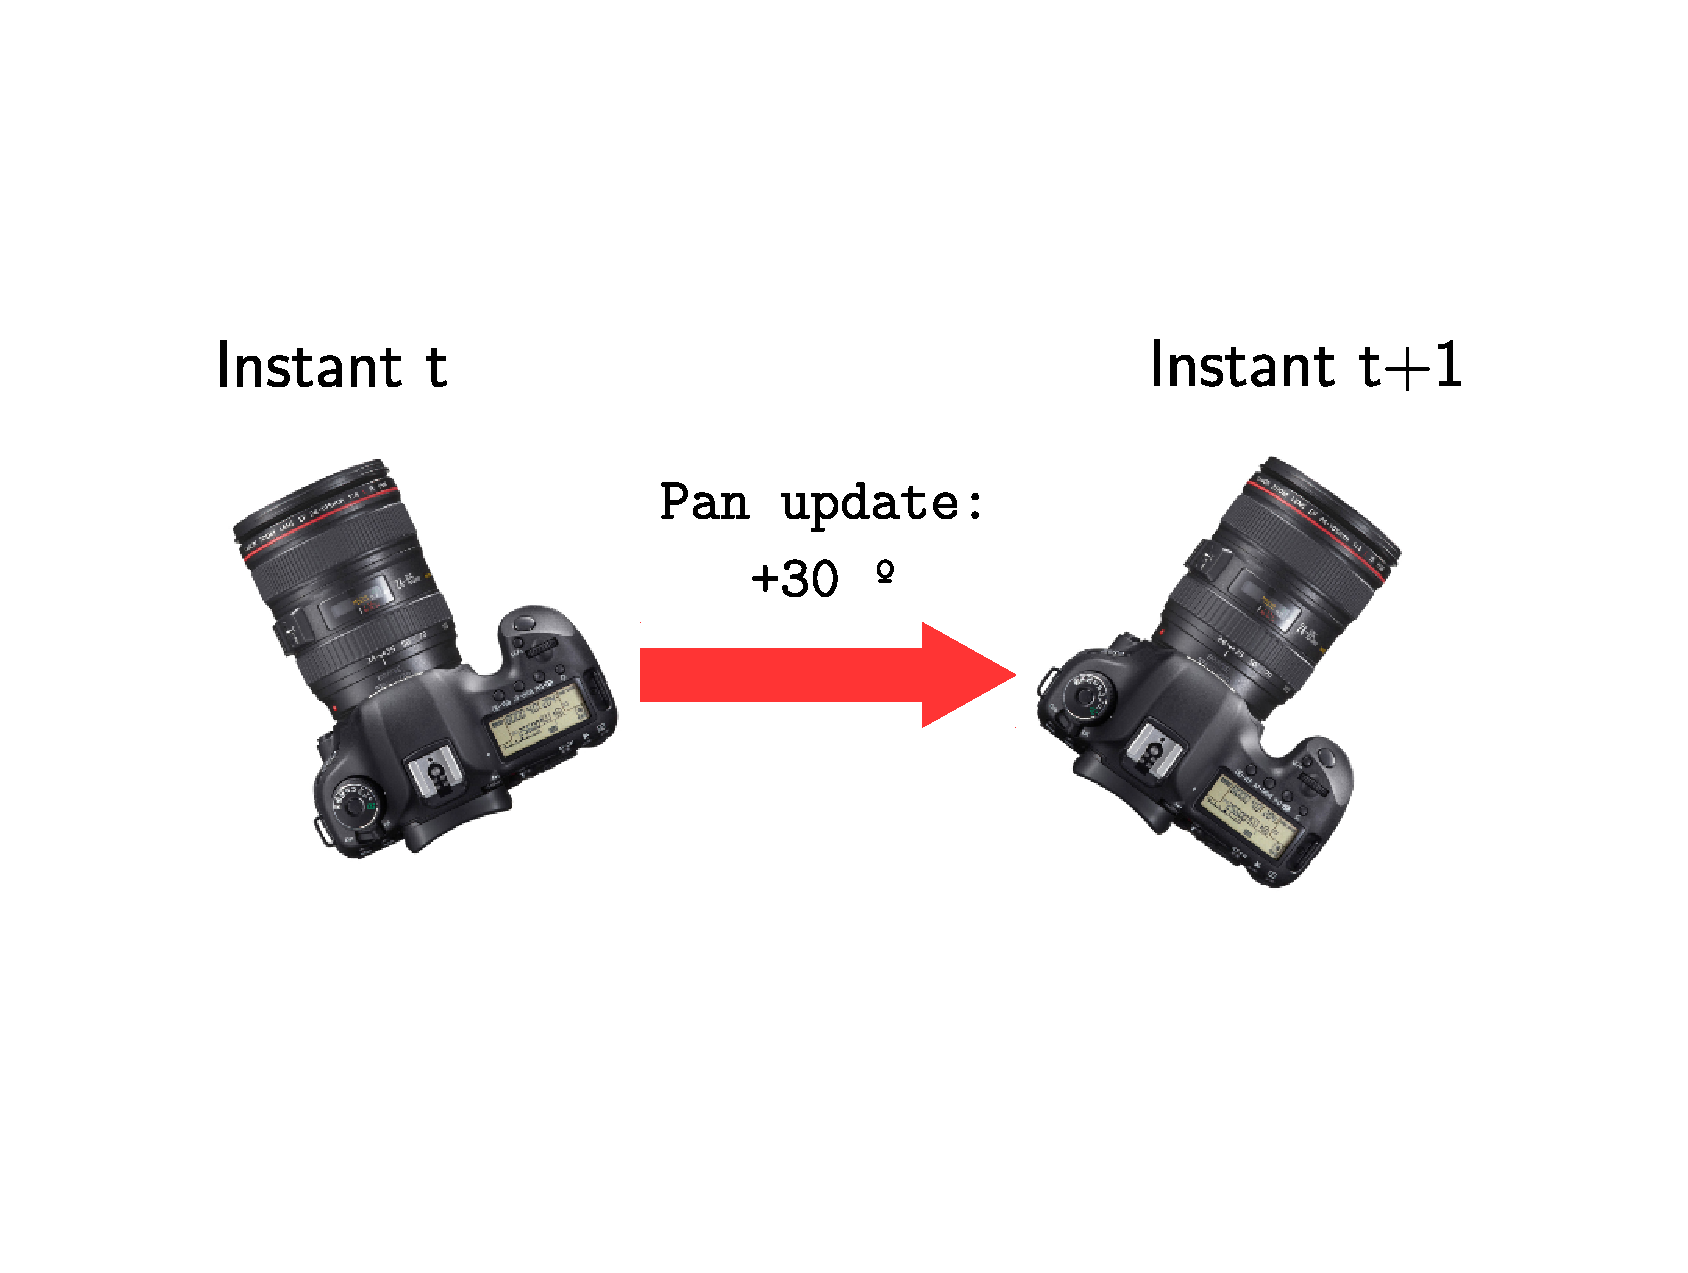
\includegraphics[width=2.7in]{images/ptz_wrong_movement}
				\caption{Wrong motion update (too long movements).}
				\label{fig:3_ptz_wrong}
			\end{subfigure}
			\qquad
			\begin{subfigure}[h]{0.4\linewidth}
				\centering
				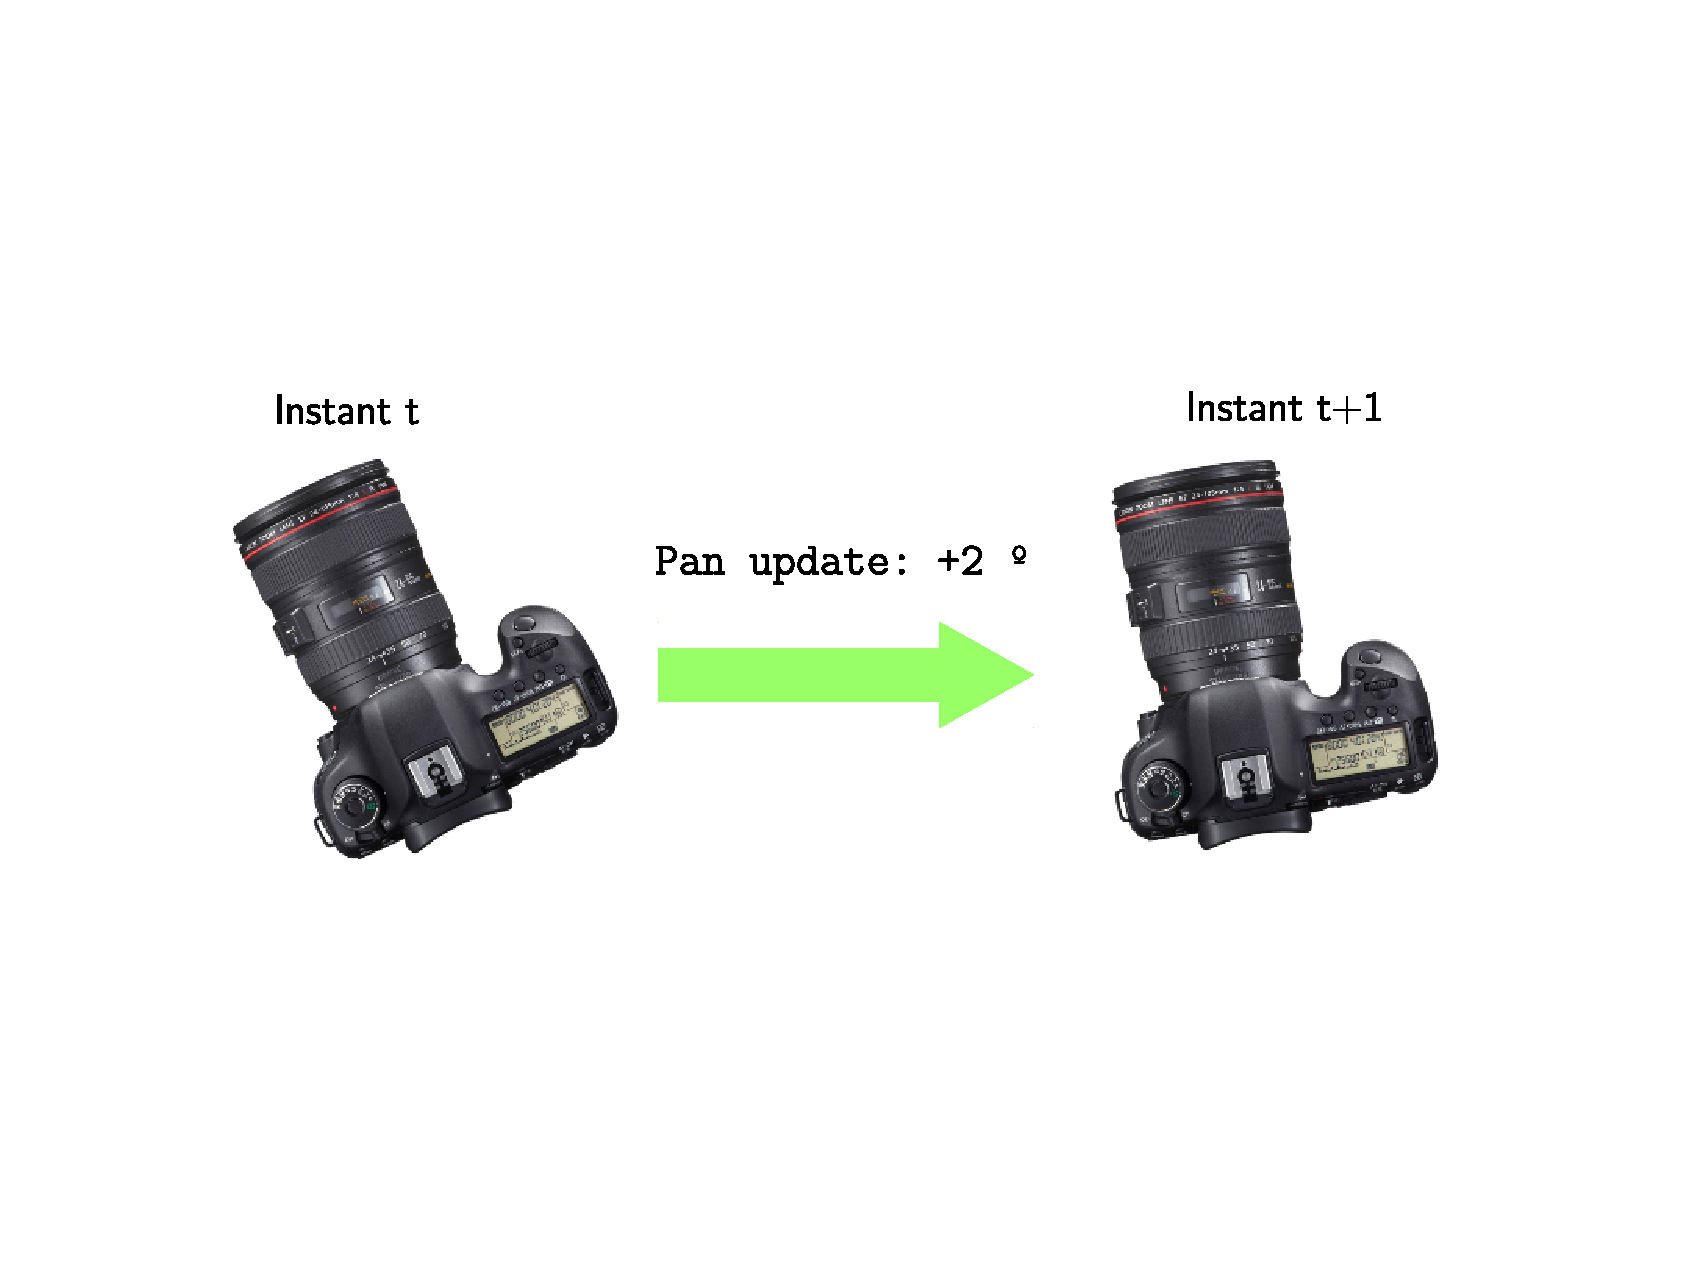
\includegraphics[width=2.7in]{images/ptz_correct_movement}
				\caption{Correct motion update (short differential movements).}
				\label{fig:3_ptz_right}
			\end{subfigure}
			\caption{Comparison between possible approaches for Pan/Tilt angle updates.}
			\label{fig:3_ptz_movements}
		\end{figure}
		

		This was the device we used for our first approximation to the sensing+actuating node (\autoref{sec:follow_ptz}), where the only response was moving the camera.\\

	\subsection{Asus Xtion Pro Live}
		It is a RGBD (RGB + Depth) sensor, designed by Asus for interactive PC applications development purposes. \\

		It has been our image source in the sensing+actuating node (\autoref{sec:follow_turtlebot}) we have developed. We used it in the second approximation (the response was the movement of the entire robot).

		\begin{figure}[h]
			\centering
			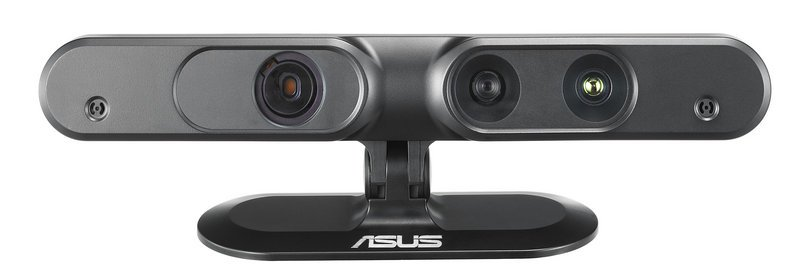
\includegraphics[width=0.4\linewidth]{images/xtion}
			\caption{Asus Xtion Pro Live. IR emitter (left), and RGB and IR lenses (right).}
			\label{fig:3_xtion}
		\end{figure}

		It counts on the left side with an IR (\emph{infrared}) light emitter, which radiates beams like a conventional light bulb (that's its function).\\

		On the right side, we can find two sensors:
		\begin{itemize}
			\item \emph{RGB sensor:} a conventional digital camera, with a resolution up to 1280x1024 px.
			
			\item \emph{Depth sensor:} it is capable of measure distance to objects, by receiving the reflections of the IR beams that we have mentioned above. It maps, for each pixel, the distance to that reflection (in mm), stored as a 16-bit long value.\\
			
			Thus, we can obtain a depth image, with a resolution of 640x480 px (@ 30 fps).
		\end{itemize}
		
		As it can be seen on \autoref{fig:3_xtion}, both sensor can't physically be in the same place, so there is a little discrepancy between both computed images:

		\begin{figure}[h]
			\centering
			\begin{subfigure}[h]{0.4\linewidth}
				\centering
				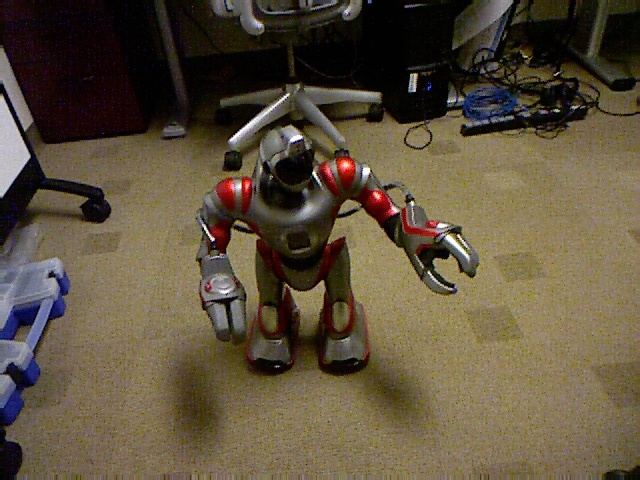
\includegraphics[width=3in]{images/rgb_before}
				\caption{RGB image.}
				\label{fig:3_rgb_bef_reg}
			\end{subfigure}
			\hfill
			\begin{subfigure}[h]{0.4\linewidth}
				\centering
				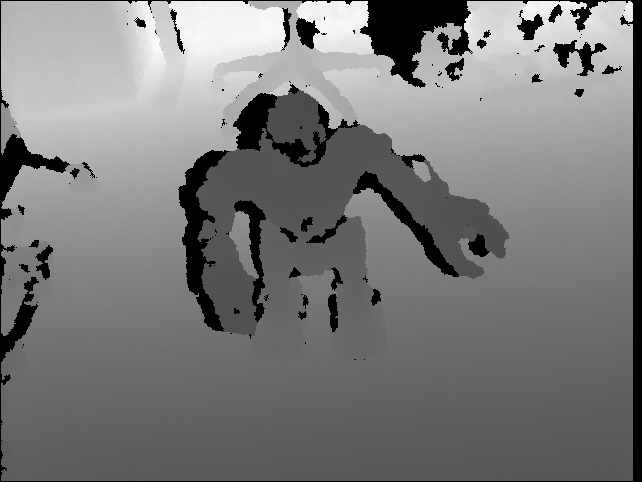
\includegraphics[width=3in]{images/depth_before}
				\caption{Depth image.}
				\label{fig:3_depth_bef_reg}
			\end{subfigure}
			
			\begin{subfigure}[h]{0.9\linewidth}
				\centering
				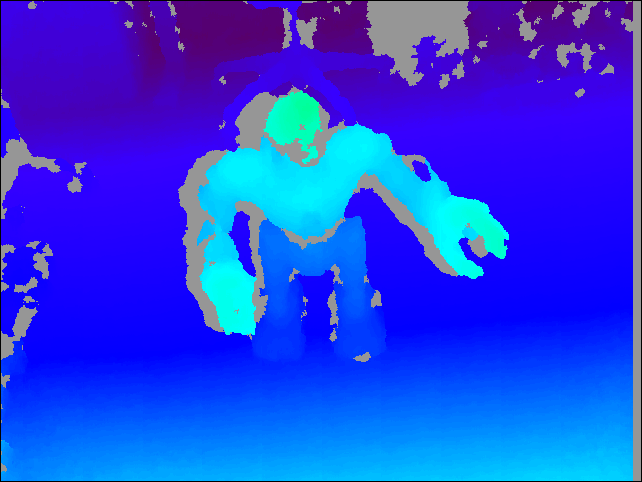
\includegraphics[width=3in]{images/disparity_before}
				\caption{Disparity (difference) between \ref{fig:3_rgb_bef_reg} and \ref{fig:3_depth_bef_reg}.}
				\label{fig:3_disparity_bef_reg}
			\end{subfigure}
			
			\caption{Both images sensed by the Xtion cameras, and the disparity between them \emph{before} the registration process.}
			\label{fig:3_bef_reg}
		\end{figure}
		
		With the goal of paliating this disparity, a process called \emph{registration} is executed for every new incoming depth image. It consists of a projection of the depth pixels into the RGB image, trying to align on an optimum way each pixel with its counterpart on the RGB image. We can observe that this can cancel to some degree the difference between both images (\autoref{fig:3_aft_reg}).
		
		
		\begin{figure}[h!]
			\centering
			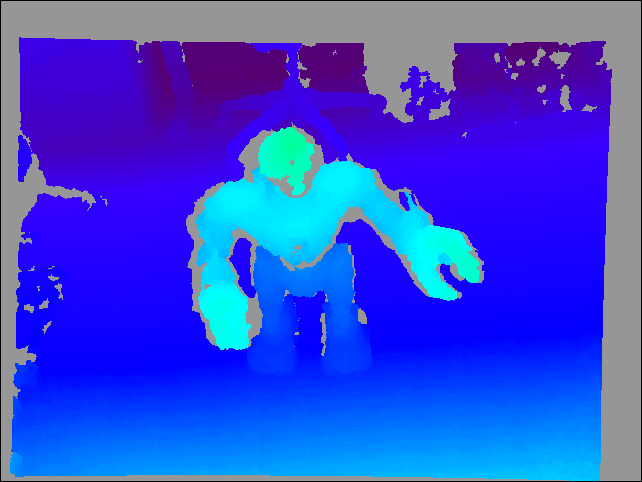
\includegraphics[width=3in]{images/disparity_after}
			\caption{Disparity between the images \emph{after} the registration process.}
			\label{fig:3_aft_reg}
		\end{figure}
		
		If we compare the new disparity (\autoref{fig:3_aft_reg}) with the previous disparity (\autoref{fig:3_disparity_bef_reg}), we can appreciate that now, the RGB and Depth images are aligned on an improved way, as if both sensors were on the same place, or much closer at least.\\
		
		So, from now on, we will call \emph{depth image} to the registered version of the depth map, as the unregistered image is not useful anymore.\\
		
		At last, we will make a mention to the open source drivers\footnote{\url{https://structure.io/openni}}, OpenNI (\emph{Open Natural Interaction}). They were originally developed by the Kinect developer company PrimeSense (which designed the Xtion device beside Asus).\\
		
		This interface allows to perform all the processes involved into handling this device (image grabbing, depth registration, etc.).
		
	\subsection{Turtlebot 2}
		The Turtlebot platform has been our main actuation platform on the developed actuation+response node (\autoref{chap:followperson}).\\
		
		\begin{figure}[h]
			\centering
			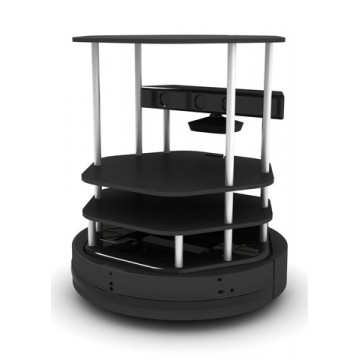
\includegraphics[width=3in]{images/turtlebot}
			\caption{Turtlebot development kit.}
			\label{fig:3_turtlebot}
		\end{figure}
		
		It is a research platform, composed by a structure jointed to a Kobuki robot (mobile base)\footnote{\url{http://kobuki.yujinrobot.com/about2/}}. Into this structure, there are also attached an Asus Xtion sensor (recently described), and a laser sensor, which has not been used on this project (nevertheless, it could be a continuation, as a navigation algorithm could be added to this project, on a similar way than in \cite{rocapal}).\\
	
		The user has the capability of connecting each of these devices via USB to the laptop, and place it at the top platform of the robot. From there, the computer can run the algorithm and command the movements. Every component can be handled with the respective ROS driver (which will be described later).
	

\section{Python}
	According to the official definition from \cite{python}, Python is \textit{an interpreted, object-oriented, high-level programming language with dynamic semantics}. It was created in 1991 by Guido van Rossum (who consecrated its name to the TV series \textit{Monty Python}). However, due to the increasing growth of \emph{Machine Learning} that happened the last two decades, it has become the most popular language for this purpose, due to its focus on \emph{easiness}, its duck typing\footnote{This refers to Python guessing about your variables, coming from the phrase \textit{''if it looks like a duck and sounds like a duck, chances are it's a duck."}} and its strong Object Orientation: everything can be treated as an object on this language. This is a very interesting feature, as it facilitates features as sharing memory, abstract processes, and much more.
	
	And, of course, it is \textit{Open Source}, so it is always under community improvements, and there are a vast number of incredibly useful third party libraries, which are impossibly easier to deploy onto your code.\\
	
	This makes this language a really potential candidate for the applications to develop (and that's precisely the reason that explains its huge growth on the software market).\\
	
	For our target, we will use Python on its version $2.7$. Although it is a relatively old version of the language, it is necessary to mantain the compatibility with ROS (\autoref{sec:3_ros}) bindings, which have not still taken the leap to the newest major version ($3.x$) on Python.\\
	
	Nevertheless, we want to mention the fact that Python is an \emph{interpreted} language, which means that its sentences are projected on another program (the Python interpreter, which executes them), and not directly by the processing hardware (CPU/GPU). This can be a con, as it makes the code execution much slower, in comparison with standard \emph{compiled} languages, which are run directly as processes, and taken by the computer hardware for its execution (as C, C++, Picky, etc.).

\section{ROS}
	\label{sec:3_ros}
	As it is said on \cite{ros-intro}, \emph{ROS} (Robot Operating System) is \textit{an open-source, meta-operating system for your robot}, maintained by the \emph{OSRF} (Open Source Robotics Foundation). It is a framework that provides a distributed, easily-scalable environment of \emph{nodes}. These nodes are programs which are independently running on the computer (or distributed over a P2P network), so they can perform individual tasks. However, they can communicate between themselves on a synchronous way (over \emph{services}, implementing a client-server role system between nodes), or on an asynchronous way, via \textbf{topics}, which will be the main benefit we will take advantage of. These topics, which rely on a standard TCP/UDP communication between sockets via the \texttt{loopback} interface, are intended for an unidirectional, streaming communication, where a node can take a role: \emph{publisher} (if it is writing data inside the topic), or \emph{subscriber} (if it is reading the data that publishers are broadcasting into the topic). The data flow through the topic, however, is not unrestricted. It must follow a ROS specific syntax, the \emph{Message} type, which is strictly defined for the communication purpose (geometry, sensoring, etc.).\\
	
	For our project we will be using the 2016 \textit{LTS} (Long Term Support) version, called \textit{Kinetic Kame}\footnote{\url{http://wiki.ros.org/kinetic}}. This is the version bundled on the installation of JdeRobot\footnote{\url{https://jderobot.org/Installation}}.\\
	
	ROS provides libraries and bindings for C++, Lisp, and \textit{Python} (\texttt{rospy}). They allow, among plenty of other stuff, to really easily set up a topic between two or more programs, which will be seen as ROS nodes.\\
	\begin{figure}[h]
		\begin{lstlisting}
...
import rospy
from std_msgs.msg import String
...
rospy.init_node('listener')              # Starting the node entity.
rospy.Subscriber('chatter', String)      # Instantiation of the topic subscriber.
rospy.spin()                             # 'Infinite loop' listening to the topic.
...
		\end{lstlisting}
		\caption{Simple stablishment of a listener node through \texttt{rospy} (code from \cite{listener-rospy}).}
		\label{fig:3_rospy_listener}
	\end{figure}
	
	However, this topic communication will be abstracted on our project by the \texttt{comm} library, as it will be seen on \autoref{sec:3_comm}.\\
	
	ROS also provides a Debian package, called \texttt{rosbash}, which allows to, in a very handy way, manage nodes and packages from a standard \texttt{bash} shell. The most remarkable feature for us is the command \texttt{roslaunch}, that launches a ROS node with a certain specific settings, configurable via a \texttt{.launch} file (which follows a XML formatting). An example for the file structure can be found on \autoref{fig:3_launch_file}.\\
	
	\subsection{\texttt{usb\_cam}}
	\label{sec:3_usb_cam}
		ROS node that creates a topic and publishes into it the digital video data incoming from a USB camera, into the topic \texttt{/usb\_cam/image\_raw}.\\
		
		This node will be used on the first approach to the sensing+actuating node (\autoref{sec:follow_ptz}), with the purpose of retrieving images from the Sony EVI D100P camera (\autoref{fig:3_evi}). In consequence, a custom configuration file\footnote{\url{https://github.com/RoboticsURJC-students/2017-tfg-nacho\_condes/blob/master/resources/usb\_cam-test.launch}} is required. We can have a glance on that configuration file (\autoref{fig:3_launch_file}).\\
		
		\begin{figure}[h]
			\centering
			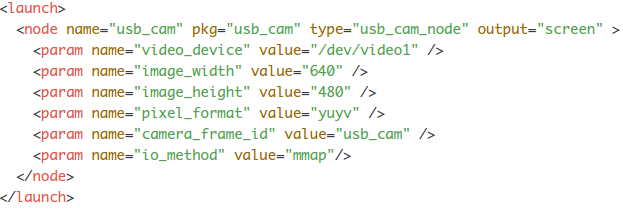
\includegraphics[width=5in]{images/usb_cam_test}
			\caption{Example of \texttt{usb\_cam-test.launch} configuration file for a ROS node.}
			\label{fig:3_launch_file}
		\end{figure}
		\begin{center}
			Usage: \texttt{roslaunch usb\_cam-test.launch}
		\end{center}

	\subsection{\texttt{openni2\_launch}}
		This ROS binding \cite{openni2-doc} provides the launch files for the \texttt{rgbd\_launch} node. This node publishes on several topics the RGB+D images provided by the Asus Xtion (\autoref{fig:3_xtion}), performing at the same time the registration process.\\
		
		This node will be used on the second iteration of the sensing+actuating node (\autoref{sec:follow_turtlebot}). It will connect the Xtion sensor to the component, providing the real-time imaging through the topic.\\

		\begin{center}
			Usage: \texttt{roslaunch openni2\_launch openni2.launch}
		\end{center}
		

	\subsection{\texttt{kobuki\_node}}
		This ROS package contains a bunch of launch files. Among them there is the one we will use: \texttt{minimal.launch}, which starts the \emph{nodelet}\footnote{A ROS nodelet performs multiple simultaneous processes, and consequently opens several topics.} that gives us the total control of the Kobuki robot connected to the computer\footnote{We refer to the robot as \emph{Kobuki} now because the mobile base of the Turtlebot (\autoref{fig:3_turtlebot}) is the only ROS device which we will control in our application.}.\\
		
		This node will be used on the second iteration of the sensing+actuating node (\autoref{sec:follow_turtlebot}). It will connect the Turtlebot motors to the component, providing the topic to command movements to them.
		
		\begin{center}
			Usage: \texttt{roslaunch kobuki\_node minimal.launch}
		\end{center}

	
\section{JdeRobot}
	As described in \autoref{sec:dl_jderobot}, JdeRobot\footnote{\url{https://jderobot.org}} is a distributed development platform/middleware, born in \cite{jmplaza-phd}. It stands out mainly for two key aspects:
	\begin{itemize}
		\item \textit{Hardware abstraction:} it behaves as an intermediate layer between control software (written by the programmer) and hardware, which can be a real device (a robot, drone, camera, laser scanner, etc.), or a simulation (on the open source world simulator Gazebo\footnote{\url{http://gazebosim.org/}}). This way, the bidirectional flow (information from sensors, and commands from the computer) is sent the same way, \textit{no matter the kind of the robotic device}.
		
		As well, this abstraction layer allows various computers to interact simultaneously with the hardware, as the communications are also abstracted to ROS topics or ICE endpoints (it will be properly explained at \autoref{sec:3_comm}), where a program has to just listen/talk to be in on. This provides a very valuable \textit{software and hardware scalability to the platform, and to the developed programs}.\\
		
		Let's have a look on a possible example on the \autoref{fig:3_jderobot_hal}. This could represent an scenario where somebody wants to virtually test a navigation algorithm. Thus, in the \emph{Computer 1}, a reactive controller is running, sensing the environment through a real laser scanner and a RGB camera (as in the work developed at \cite{rocapal}). This controller receives data from the sensors, computes a proper navigation response, and sends it to a virtual robot, simulated on Gazebo.
		
		Additionally, another machine (\emph{Computer 2}) is running a viewer, which allows it to draw the images seen by the camera, and the laser readings from the scanner. So, this component only receives the data from the sensors, and does not send any kind of data to the devices.
		
		We can see that both components can perfectly run together and on different machines, even when they are written over completely different languages (Python and C++, respectively). In addition, we can perfectly handle virtual and real devices simultaneously, even if they talk through different interfaces (ROS or ICE), due to the perfect support of this division by the \texttt{comm} (\autoref{sec:3_comm}) library.\\
		
		
		\begin{figure}[h!]
			\centering
			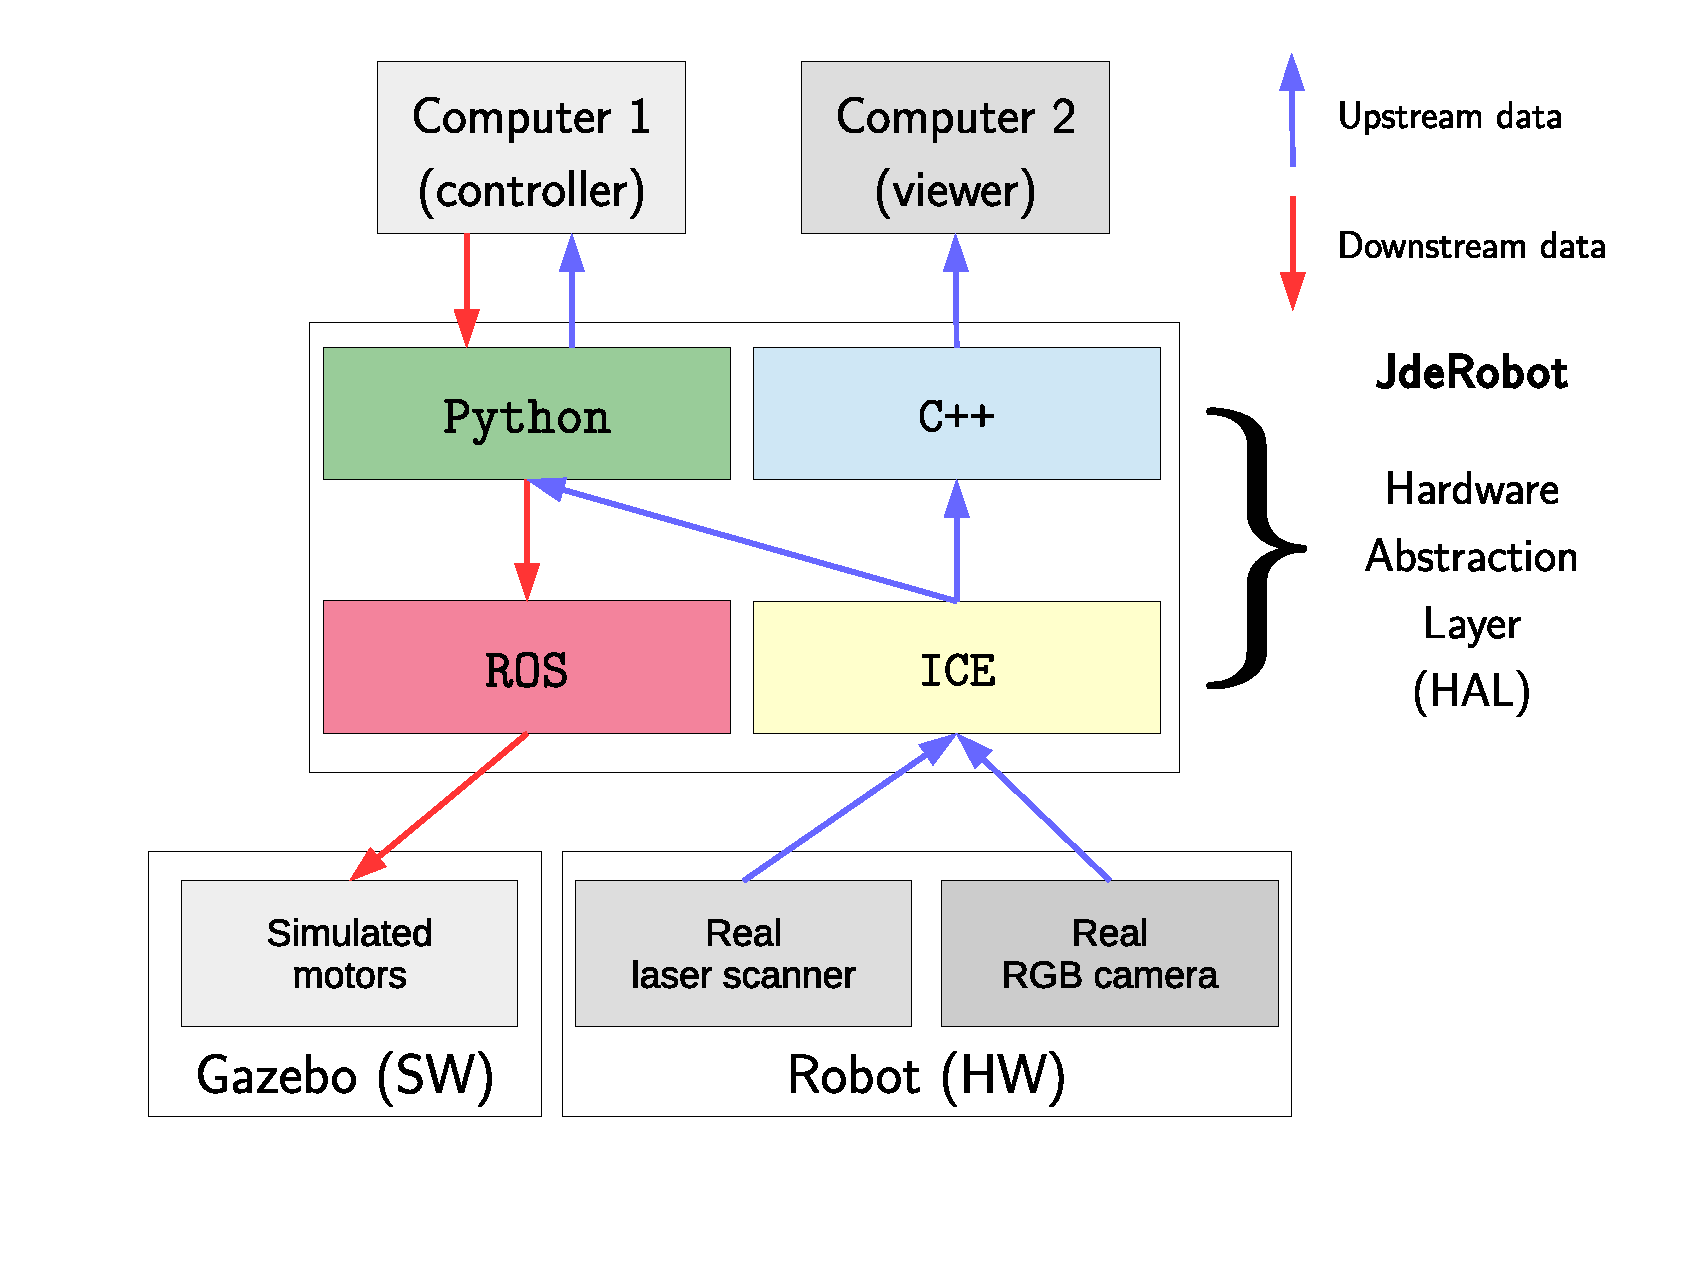
\includegraphics[width=4in]{images/jderobot_hal}
			\caption{JdeRobot abstraction layer, and a possible use distributed, multi-middleware scenario.}
			\label{fig:3_jderobot_hal}
		\end{figure}
		
		 \textit{So, in this easiness and flexibility resides the main advantage of using JdeRobot}.
		
		\item \textit{Wide device support:} JdeRobot provides full compatibility with ROS Kinetic Kame, so it can perfectly integrate with ROS Nodes (in our concern, we can communicate with the Turtlebot and the Xtion devices via several topics that the ROS intermediate nodes open).
		
		\item \textit{Behavioral based on threaded parallel schemes:} as it is introduced at  \cite{jmplaza-phd}, inside a component, we will find one or more \emph{schemes}, objectified on threads. These threads run concurrently with an specific timing (so it does not overload the CPU in vain if a few iterations per second are enough for a vivacious and correct response).\\
		
		These schemes perform different tasks each, as seen on \autoref{fig:2_tasks} on a non-blocking way, and share memory. This has been followed on a comfortable way on our implementation: the threads are independent, but the tasks they control are performed by Python objects, which are interconnected between them:
		
		As an example, we can see how this has been performed inside our Python code:
		
		\begin{figure}[h]
			\centering
			\begin{lstlisting}
...
cam = Camera(ros_topic)           # Creation of the camera.
net = Network(graph_model)        # Creation of the CNN.

net.setCamera(cam)                # Connection of the camera and the CNN,
                                  # which now can share memory.

t_cam = ThreadCamera(cam)         # Instantiation and start of the thread which
t_cam.start()                     # implements the Camera schema.

t_net = ThreadNetwork(net)        # Instantiation and start of the thread which
t_net.start()                     # implements the Network schema.
...
			\end{lstlisting}
			\caption{Handling schemes on Python with objects and threads.}
			\label{fig:3_schemes_python}
		\end{figure}
	\end{itemize}
	
	\vspace{0.4in}
	
	To sum up, we have described the goodness of the JdeRobot framework for our purposes, and seen how we can implement the \textit{useful schemes paradigm} on an easy way into Python, our development language.\\
	
	Now, in the next subsections, we will examine which of the JdeRobot components, apart of the structure, have been of greatest interest for us.
	
	\subsection{Digit Classifier}
	\label{sec:3_digitclassifier_jderobot}
		This JdeRobot component\footnote{\url{https://github.com/JdeRobot/dl-digitclassifier}} was originally designed by David Pascual \cite{dpascualhe} and Nuria Oyaga \cite{noyaga}, and it was used on this project to land on the concept of neural networks.\\
		
		Its design aims to \textit{classify handwritten numbers} with the use of a Convolutional Neural Network (\autoref{sec:1_cnn}), that classifies the incoming images from a video source.\\
		
		\begin{figure}[h]
			\centering
			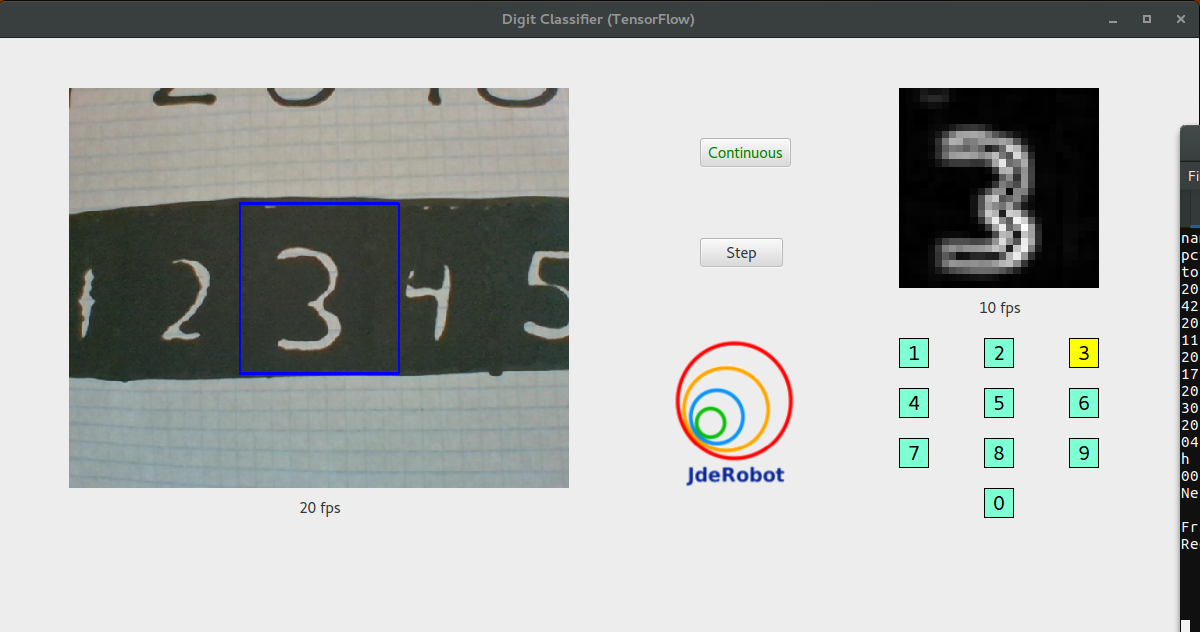
\includegraphics[width=4in]{images/digitclassifier}
			\caption{\texttt{DigitClassifier} on action.}
			\label{fig:3_digitclassifier}
		\end{figure}
		
		The previous implementations were written in Keras and Caffe (Python libraries to implement Neural Networks), so we made the same on TensorFlow (\autoref{sec:3_tensorflow}), to accomplish an initial domain of this Machine Learning framework.\\
		
		The implementation of this convolutional neural network consists on a concatenation of layers, following the scheme shown on \autoref{fig:3_digitclassifier_neural_structure}, which perform specific operations.
		
		\begin{figure}[h]
			\centering
			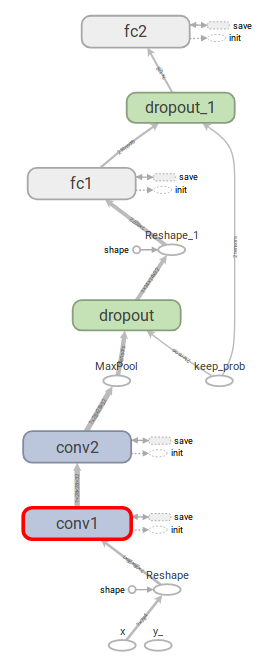
\includegraphics[width=2in]{images/digitclassifier_network_graph}
			\caption{Digit classifying neural structure.}
			\label{fig:3_digitclassifier_neural_structure}
		\end{figure}



		\begin{enumerate}
			\item \texttt{conv1}: first convolutional layer. As described in \autoref{sec:1_cnn}, it performs a 2D convolution between a $5px \times 5px$ square mask\/kernel (\texttt{W\_conv1}), and then adds a bias/intercept term (\texttt{b\_conv1}).\\
			\item \texttt{conv2}: second convolutional layer. It performs the same operation taking the output from the previous layer as an input, using a different weights mask and bias terms.\\
			
			Until now, what we have done is extracting patterns on each digit type (e.g. discovering typical circles on $0$ and $8$, which are always present on the same zone of the image).\\
			\item \texttt{pooling}: as the activation maps can be growing in size as we perform feed forward propagation, a \emph{pooling} operation is performed. It consists on sampling the input. Concretely, we retain the \textit{maximum} value for each 2 pixels, which is known as \textit{$2x2$ \texttt{max pooling}}
			
			\item \texttt{dropout}: this layer does not strictly perform any mathematical operations. It lets pass the TENSORS through it, but randomly switching off some neurons. This is parameterized by a user input, using a variable called \texttt{keep\_prob}. In our case, we set it to $0.5 (50\%)$ during the training process, to avoid overfitting by forcing the network to modify the neural paths randomly, as not every neuron is available on every moment. This is kind of similar to augmenting the dataset during the training process. The rest of the time (when the network is used to make inferences), this parameter is set to $1.0$, which means that no neurons are switched off at all.\\
			\item \texttt{fc1}: first fully connected layer. These layers, also known as \emph{dense} layers, are distinguised because every neuron is connected to every activation from the previous layer. So, this kind of layers are used for \text{pattern association with labels}, due to the relationship they can infer between every input.\\
			\item \texttt{fc2}: the output layer. It connects all the outputs of the previous dense layer and groups the output in a 10-dimensional vector, which contains the probability of the digit to belong to each one of the possible classes.
		\end{enumerate}


		
		Once all this was achieved, we upgraded the code (from single ICE support to ROS+ICE via the \texttt{comm} library), and unified it (Keras + TensorFlow frameworks in a single component, under choice using the YML configuration file) on the official JdeRobot repository. From there it can be used right out of the box with the included model for both frameworks. In addition, you can train your own models using the provided datasets, or yours if you build another.
	
	
	\subsection{\texttt{evicam\_driver}}
	\label{sec:3_evicam_driver}
	This driver, bundled into JdeRobot\footnote{\url{https://github.com/JdeRobot/JdeRobot/tree/master/src/drivers/evicam\_driver}}, allows the user to send movements commands to a Sony EVI D100P camera \autoref{fig:3_evi}) and retrieve information from it, creating an ICE endpoint that is ready to interact with the camera \emph{PT} (Pan, Tilt) motors.\\
	
	As this is a low-level driver, written in C++, it requires to be used on a specific way, which has been documented\footnote{\url{https://jderobot.org/Handbook\#PanTilt_Teleop}} to be easily applied in the future.\\
	
	This driver defines an interaction API with the camera, which allows us to get the values from the motors encoders:
	\begin{lstlisting}
import config
import comm
...

cfg = config.load('yml_configuration_file')
jdrc = comm.init(cfg, 'NodeName')


# Instantiation for the motors:
PTMotors = jdrc.getPTMotorsClient('NodeName.PTMotorsEndpoint')

print(PTMotors.getLimits()) # Shows the max/min values for pan, tilt 
                            # and each speed.

print(PTMotors.motors.data) # Shows the current values for pan, tilt
                            # and each speed.

# Let's move the camera! As easy as:
PTMotors.setPTMotorsData(new_pan, new_tilt, max_pan_speed, max_tilt_speed)
	\end{lstlisting}
	
	\subsection{\texttt{comm}}
		\label{sec:3_comm}
		\texttt{comm} is the basic library to perform communications between different components. It is what supports all the data flows in a typical scenario (\autoref{fig:3_jderobot_hal}).\\
		
		\texttt{comm} consists on a collection of bindings to easily create a link between two components, or between a device and a component. On the lowest level, we can use it relying on ROS (through topics as it was explained before on \autoref{sec:3_ros}), or through an ICE proxy. ICE\footnote{\url{https://zeroc.com/products/ice}} is an object-oriented middleware that, in our purpose, allows to abstract a data flow to a TCP/IP endpoint (an address/hostname, and a port), which can even support a communication between two or more programs inside the same machine.\\
		
		To create a communicator with \texttt{comm}, it needs the specification for that link (underlying middleware, topic/endpoint, etc.), so it uses the JdeRobot standard: YML\footnote{Legible data serialization format.} configuration files, which can be like in \autoref{fig:3_yml_format}.
		\begin{figure}[h]
			\centering
			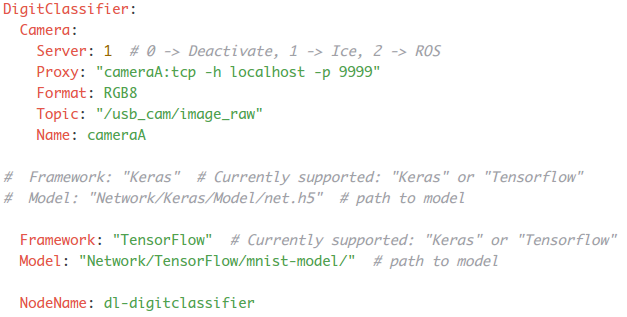
\includegraphics[width=4in]{images/yml_format}
			\caption{YML format on the \texttt{digitclassifier.yml} file.}
			\label{fig:3_yml_format}
		\end{figure}
		
\section{OpenCV}
\section{TensorFlow}
\label{sec:3_tensorflow}
\section{Keras}
\section{PyQt (v.5)}
\section{Threading}
